\chapter{Diskussion}\label{chap:d}
Die Diskussion analyisiert die Resultate der Methode (siehe \doubleref{chap:m}),
um daraus eine Antwort auf die Fragestellung zu bilden. Zu diesem Zweck werden
einige allgemeine Feststellungen getroffen und die Unterfragen beantwortet
(siehe \doubleref{chap:d_frage}). Im zweiten Teil der Diskussion folgt ein Fazit,
ein Ausblick (siehe \doubleref{chap:d_faz-aus}), und eine Selbstreflexion (siehe
\doubleref{chap:d_reflex}). Dabei verschiebt sich der Fokus von der Fragestellung
weg und auf eine allgemeinere Betrachtung der Arbeit.


\section{Fragestellung und Unterfragen}\label{chap:d_frage}
Die Fragestellung und die Unterfragen decken nicht alle Erkenntnisse aus den
Resultaten ab (siehe \doubleref{chap:r}). Einige allgemeine Feststellungen geben
Einblick, wie die Resultate  zu verstehen sind. 

Die Grund-Basis Version und die Grund-Speed Version (siehe
\doubleref{chap:m_auswert}) erreichen in allen Kriterien für alle Datensets die
beste Leistung. Die Resultate zwischen den Versionen sind dabei bis auf den Wert
des Kriteriums der Geschwindigkeit (siehe \doubleref{sub:m_eval_speed}) fast
ununterscheidbar. In diesem Kriterium erreicht die Grund-Speed Variation leicht
bessere Werte als die Grund-Basis Version. Beispielsweise stellt die Grund-Speed
Version Zeichnungen aus dem Quickdraw Datenset durchschnittlich vier Schritte
früher als die Grund-Basis Version fertig. Insgesamt erreicht somit die
Grund-Speed Version die beste Leistung. Unter den Versionen, die auf der
physikalischen Umgebung basieren, erreichen Ebenfalls die Physik-Basis und die
Phyisk-Speed Versionen die beste Leistung. Die Werte sind allerdings deutlich
tiefer als bei der Grund-Basis und der Grund-Speed Version.

Die Grund-MNIST Version und die Physik-MNIST Version sind in allen Kriterien
schlechter als die Basis und Speed Versionen. Auch im Kriterium der
Erkennbarkeit (siehe \doubleref{sub:m_eval_rec}) von MNIST Ziffern bringt die
MNIST Variation keinen Vorteil. Die Physik-MNIST-Speed Version erbringt
insgesamt die schlechteste Leistung. Eine Erklärung dafür ist, dass diese
Version eine Kombination von allen Variationen (siehe \doubleref{chap:m_var})
ist und somit von der leistungsstarken Grund-Basis Version am stärksten
abweicht.


\subsection{Beantwortung der Unterfragen}\label{sub:d_frage_unter}
Insgesamt sechs Unterfragen werden beantwortet (siehe \doubleref{chap:einleit}).
Diese Unterfragen weiten die Fragestellung aus und tragen zu der
schlussendlichen Antwort auf die Fragestellung bei. Die Antworten beruhen auf
den Resultaten, aber auch auf Erkenntnissen aus der Methode selbst (siehe
\doubleref{chap:m}).

\subsubsection*{Wie kann die Architektur einer KI aussehen, die das Nachzeichnen erlernt?}\label{subsub:d_frage_unter_1}
Unter der Annahme, dass die KI dieser Arbeit das Nachzeichnen erlernt, (siehe
\doubleref{sub:d_frage_frag}), kann die Architektur genau so aussehen, wie sie in
dieser Arbeit beschrieben ist (siehe \doubleref{sub:m_grund_dood}).

\subsubsection*{Wie lässt sich die Leistung der KI in ihrer Aufgabe
beurteilen?}\label{subsub:d_frage_unter_2} Die Leistung der KI lässt sich durch
die definierten Kriterien (siehe \doubleref{chap:m_eval}) beurteilen. Das
Kriterium Der Übereinstimmung ist durch einen objektiven und absoluten Wert
repräsentiert, wodurch es das aussagekräftigste Kriterium ist. Ausserdem ist der
maximale Wert des Kriteriums ($100\%$) unabhängig vom gezeichneten Bild und dem
Verhalten der KI. Dadurch ist das Kriterium geeignet für Vergleiche zwischen
Versionen der KI.

Die Kriterien der Erkennbarkeit und der Geschwindigkeit sind an subjektive
Annahmen gebunden. Zum Beispiel wird für das Kriterium der Geschwindigkeit ein
subjektiver Punkt der Fertigstellung definiert (siehe
\doubleref{sub:m_eval_speed}). Dadurch sinkt ihre Aussagekraft. Allerdings
verändern sich die Annahmen nicht und die Kriterien sind in jedem Fall durch
einen Zahlenwert repräsentiert. Somit eignen sich auch diese Kriterien für
Vergleiche zwischen Versionen der KI. Aus der Annahme heraus, dass für Menschen
beim Nachzeichnen Erkennbarkeit wichtiger als absolute Genauigkeit ist, ergibt
sich das Kriterium der Erkennbarkeit als besonders wichtig. Aus diesem Grund
ist das Kriterium in der Fragestellung (siehe \doubleref{chap:einleit})
festgehalten.


\subsubsection*{Wie lässt sich die Leistung der KI in ihrer Aufgabe verbessern?}\label{subsub:d_frage_unter_3} 
Bezogen auf die definierten Kriterien erreicht die Grund-Basis Version Werte,
die durch die implementierten Variationen nicht verbessert werden. Die
Grund-Speed Version ist hierbei eine Ausnahme (siehe \doubleref{chap:d_frage}).
Insgesamt sind die meisten Variationen der KI ein gescheiterter Versuch der
Verbesserung der Leistung. Die Grund-Basis Version erfuhr allerdings während
dessen Entwicklung signifikante Verbesserungen. Die grössten Verbesserungen
stammen aus der Optimierung der Hyperparamter durch den Baysian Optimization
Algorithmus (siehe \doubleref{sub:m_grund_data}). Diese Optimierung steigerte
die Leistung der Grund-Basis Version im Kriterium der prozentualen
Übereinstimmung um fast $50\%$.

\subsubsection*{Welche Einflüsse haben physische Einschränkungen auf die
Leistung der KI?}\label{subsub:d_frage_unter_4} Die phyischen Einschränkungen,
die auf Physiksimulationen basieren (siehe \doubleref{sub:m_var_phy}),
verschlechtern die Leistung der KI bezogen auf die definierten Kriterien. Alle
Versionen, die auf der Grundumgebung basieren, erzielen höhere Werte als die
gleichen Versionen basierend auf der phyiskalischen Umgebung. Die physikalische
Umgebung hat zum Ziel, die Bewegungen der KI realistischer zu gestalten als die
Grundumgebung. In diesem Bereich kann der Einfluss nicht objektiv bestimmt
werden. Aus Beobachtungen der Bilder, welche in der physikalischen Umgebung
gezeichnet sind (siehe \doubleref{chap:r_bild}), gehen ebenfalls keine
Erkenntnisse in diesem Bereich hervor. Die Bilder unterscheiden sich nicht
bedeutend von denjenigen aus der Grundumgebung.

\subsubsection*{Wie ändert sich die Leistung der KI für Strichbilder, die im Training nicht enthalten sind?}\label{subsub:d_frage_unter_5} 
In allen acht Versionen bleibt die Leistung der KI zwischen den drei Datensets
(siehe \autoref{tab:models}) vergleichbar. Die Tabellen (siehe \autoref{tab:Grund-3-datasets} und \autoref{tab:Phy-3-datasets})
zeigen die Leistung der Grund-Basis Version und der
Physik-Basis Version in den drei definierten Kriterien, getestet auf die drei
Datensets. Der Wert der Übereinstimmung zwischen dem MNIST Datenset und dem
EMNIST Datenset ist beinahe identisch. Für beide Versionen ist der Wert der
Übereinstimmung für das QuickDraw Datenset niedriger. Insgesamt ist die KI in
diesem Kriterium jedoch kaum beeinflusst durch die Wahl des Datensets. Die
Analyse der anderen zwei Kriterien führt zu einer ähnlichen Schlussfolgerung.
Interessant ist, dass vor allem die Grund-Basis Version eine viel höhere
Geschwindigkeit im Zeichnen von MNIST Zahlen hat, als im Zeichnen von EMNIST
Buchstaben. Obwohl die Formen zu grossem Teil ähnlich sind, scheint die KI durch
das spezifische Training auf MNIST Ziffern eine höhere Geschwindigkeit zu
entwickeln.

\begin{table}[!ht]
    \centering
    \caption{Grund-Basis Leistung}\label{tab:Grund-3-datasets}
    \begin{tabular}{|l|l|l|l|}
        \hline
            ~ & Übereinstimmung \% & Erkennbarkeit \% & Geschwindigkeit \\ \hline
            MNIST & 86.5 & 86.6 & 24.5 \\ \hline
            EMNIST & 86.8 & 74.5 & 38.2 \\ \hline
            QuickDraw & 79.1 & 80.5 & 39.1 \\ \hline  
        \end{tabular}
\end{table}

\begin{table}[!ht]
    \centering
    \caption{Physik-Basis Leistung}\label{tab:Phy-3-datasets}
    \begin{tabular}{|l|l|l|l|}
        \hline
            ~ & Übereinstimmung \% & Erkennbarkeit \% & Geschwindigkeit \\ \hline
            MNIST  & 56.4 & 46.4 & 62.5 \\ \hline
            EMNIST & 57.6 & 32.4 & 63.5 \\ \hline
            QuickDraw & 48.1 & 55.7 & 63.8 \\ \hline
        \end{tabular}
\end{table}


\subsubsection*{Wie und inwiefern lässt sich das Verhalten der KI mit menschlichem Zeichnen vergleichen?}\label{subsub:d_frage_unter_6}
Die Antwort auf diese Frage leitet sich nicht aus den objektiven Resultaten ab,
sondern basiert auf subjektiven Beobachtungen. Die Bewegungen in der
Physik-Version der künstlichen Intelligenz basieren grundsätzlich auf den selben
Gesetzen wie die Bewegungen in der echten Welt. Allerdings sind die Bewegungen
stark vereinfacht im Vergleich zu menschlichen Bewegungen. Ausserdem ist für die
künstliche Intelligenz der Druck des Stiftes nicht veränderbar. Zumindest
konzeptuell nähert die künstliche Intelligenz menschliches Zeichnen,
bezogen auf die physischen Einschränkungen, an. Einige menschliche Gewohnheiten
sind bei der künstlichen Intelligenz allerdings nicht beobachtbar. Zum Beispiel
beginnt die künstliche Intelligenz beim Zeichnen von Ziffern an zufälligen
Orten, während Menschen in der Regel für jede Ziffer an der selben Stelle
ansetzen.


\subsection{Beantwortung der Fragestellung}\label{sub:d_frage_frag}
Die Fragestellung lautet: Inwiefern kann eine künstliche Intelligenz lernen,
Strichbilder auf eine physische Weise nachzuzeichnen, sodass diese durch ein
automatisches System erkannt werden? (siehe \doubleref{chap:einleit}) Diese Frage
hat mehrere Aspekte, die teilweise bereits durch die Unterfragen (siehe
\doubleref{sub:d_frage_unter}) erfasst werden. Für die schlussendliche Antwort
folgt eine genauere Ausführung der Aspekte.

Die KI zeichnet durch Physiksimulationen und durch allgemeine Einschränkungen
der Bewegungsfreiheit auf eine annähernd physische Weise. Das Zeichnen ist nur
annähernd physisch, da alle Bewegungen simuliert sind und somit in keiner
phyischen Umgebung stattfinden. Ausserdem sind die Simulationen nicht vollkommen
realistisch (siehe \doubleref{subsub:d_frage_unter_4}).

Die künstliche intelligenz erlernt das Nachzeichnen bezogen auf die Kriterien,
nach denen es definiert ist, erfolgreich. Dafür sprechen die Werte der besten
Versionen für das Nachzeichnen von Ziffern (siehe \doubleref{chap:d_frage}). Die
hohen Werte im Kriterium der Erkennbarkeit der besten Versionen bestätigen
ausserdem, dass die Zeichnungen der KI in den meisten Fällen von einem
automatischen System (einer zweiten KI) erkannt werden.

Laut der Fragestellung soll die KI das Nachzeichnen von Strichbildern erlernen.
Damit ist implizit das Nachzeichnen von allen möglichen Arten von Strichbildern
gemeint. Die Leistung der KI kann nicht auf alle möglichen Strichbilder
überprüft werden, aber der Test mit drei verschiedenen Datensets ergibt
vielversprechende Resultate (siehe \doubleref{chap:r_tab}). Die KI erlernt das
Nachzeichnen von Ziffern, Kleinbuchstaben und zehn zufälligen Motiven aus dem
QuickDraw Datenset erfolgreich. Durch die Vielfalt im QuickDraw Datenset kann
die Annahme getroffen werden, dass die KI zumindest einen grossen Teil der
denkbaren Strichbilder erfolgreich nachzeichnen kann. 

Die zusammenfassende Antwort auf die Frage lautet somit: Eine künstliche
Intelligenz kann das Nachzeichnen von Strichbildern auf annähernd physiche Weise
in dem Sinne lernen, dass die fertige Zeichnung von einem automatischen System
grösstenteils erkannt wird, die Übereinstimmung zwischen der Vorlage und der
Zeichnung gross ist und die Zeichnung nicht viel Zeit in Anspruch nimmt.

Diese Antwort bezieht sich auf die genaue Frage, wie sie in der Einleitung steht.
Der nächste Abschnitt beurteilt die Frage durch die Erkenntnisse aus dieser
Arbeit und geht auf mögliche Erweiterungen ein.


\section{Fazit und Ausblick}\label{chap:d_faz-aus} Die Resultate erlauben eine
positive Antwort auf die Fragestellung (siehe \doubleref{sub:d_frage_frag}).
Diese Antwort setzt allerdings einige Annahmen vorraus, die weiter diskutiert
werden können. Die grösste Annahme bezieht sich auf die Definition des
Nachzeichnens. Diese Arbeit definiert Nachzeichnen durch drei Kriterien und
durch physische Rahmenbedingungen. Die Kriterien sind für eine künstliche
Intelligenz sinnvoll gewählt (siehe \doubleref{subsub:d_frage_unter_2}),
allerdings wären auch andere Kriterien möglich. Nachzeichnen ist eine
menschliche Tätigkeit. Dieser menschliche Aspekt ist in den definierten
Kriterien nicht enthalten. Die zweite Annahme bezieht sich auf die Definition
eines Strichbilders. Die KI kann nur eine bestimmte Art von Strichbildern
nachzeichnen. Mehrfarbige Bilder kann die KI beispielsweise nicht zeichnen.

Die physischen Rahmenbedingungen unterscheiden sich von denjenigen, die ein
Mensch erfährt. Das kommt daher, dass die phyischen Rahmenbedingungen für die KI
lediglich simuliert sind. Das verunmöglicht eine umfassende Antwort auf die
Frage, ob die künstliche Intelligenz auf eine physische Weise zeichnet. Dieses
Problem könnte mit einem Roboter gelöst werden, der die künstliche Intelligenz
in eine reale, phyische Umgebung überführt. Der Roboter könnte verschiedenste
Strichbilder auf einem echten Stück Papier, und somit zwangsläufig auf physische
Weise nachzeichnen.

Aktuell sind die Bewegungen der künstlichen Intelligenz in
gewissen Belangen eingeschränkt. So ist beispielsweise die Druckstärke nicht
variierbar. Ausserdem zeichnet die künstliche Intelligenz vorwiegend kleine
Strichbilder. Experimente mit grösseren Konstrukten, wie ganze Wörter, wären
eine mögliche Erweiterung. 

Alles in allem sind eine Vielzahl an denkbaren Fragen und Ideen möglich, die auf
ReSketch, der künstlichen Intelligenz hinter dieser Arbeit, basieren.


\section{Selbstreflexion}\label{chap:d_reflex} Die Selbstreflexion gibt genauere
Einblicke in die Vorangehensweise hinter dieser Arbeit. Diese Dokumentation ist
grundsätzlich eine Zusammenfassung der wichtigsten Ereignisse. Viele Aspekte
bleiben verschwiegen. Die Selbstreflexion geht näher auf drei wichitige Aspekte
ein, die in der zusammengefassten Dokumentation nicht genug betont sind.

Die Dokumentation ist mit LaTeX und spezifischer der ETH Thesis Formatvorlage
\cite{noauthor_cadmo_2014} formatiert. Ein Grossteil der Abbildungen stammt von
den Autoren und ist in Adobe Illustrater oder der Python Library Matplotlib
erstellt.

\subsection{Optimierung der KI}\label{sub:d_reflex_opti} Insgesamt sind acht
Versionen der KI präsentiert. Im Verlaufe des Projektes gab es viele weitere
Versuche, die Leistung der künstlichen Intelligenz zu verbessern. Diese Versuche
führten allerdings häufig dazu, dass die KI den akkumulierten Reward (siehe
\doubleref{sub:t_rl_func}) nicht mehr maximieren konnte. In der Dokumentation
sind deswegen nur diejenigen Versuche festgehalten, die tatsächlich
funktionieren. Häufig ist der Grund hinter dem Scheitern oder dem Erfolg einer
KI schwer zu erkennen, was die Optimierung allgemein verkompliziert.

Die Strategie hinter der Optimierung der KI besteht in den meisten Fällen aus
wiederholtem ausprobieren mit Anpassungen zwischen jedem Versuch. Hilfsmittel,
wie der Baysian Optimization Algorithmus, erleichtern diese Aufgabe massgeblich.
Diese Strategie der Optimierung ist für einen Computer sehr ressourcenintensiv.
In den längsten Optimierungsphasen liefen die beiden Computer, auf denen die
Arbeit verrichtet wurde, zusammen länger als $48$ Stunden.

\subsection{Analyse der KI}\label{sub:d_reflex_analys}
Eine Analyse der künstlichen Intelligenz ist notwendig, um die Fragestellung und die
Unterfragen zu beantworten. Aber auch während der Entwicklung ist eine
stetige Analyse nötig, um die KI zu verstehen und zu verbessern.

Die Analyse besteht hauptsächlich darin, die Leistung der künstlichen
Intelligenz zu beurteilen. Das geschieht mittels den Kriterien, die für diesen
Zweck definiert sind (siehe \doubleref{chap:m_eval}). Die Kriterien sind dabei so
definiert, dass sie für jede mögliche Variation identisch bleiben. Der
durchnittliche akkumulierte Reward ist beispielsweise absichtlich kein
Kriterium. Der akkumulierte Reward ist abhängig von der Reward-Function (siehe
\doubleref{sub:t_rl_func}) und unterscheidet sich somit zwischen Variationen.

Eine weitere Form der Analyse stammt aus der Sammlung von Daten über das
Lernverhalten der KI. So wird aus jedem Training ein Graph erstellt, der die
durchschnittliche Leistung der KI in jeder Episode erfasst (siehe
\autoref{fig:learnplot}). Die Leistung ist dabei durch den akkumulierten Reward
in jeder Episode repräsentiert. Wie erwähnt können Versionen der KI nicht anhand
ihres akkumulierten Rewards verglichen werden. Der akkumulierte Reward zeigt
allerdings für einzelne Versionen am präzisesten, inwiefern diese ihren Reward
maximieren können.

%bild Lernkurve
\begin{figure}[!ht]
    \centering
    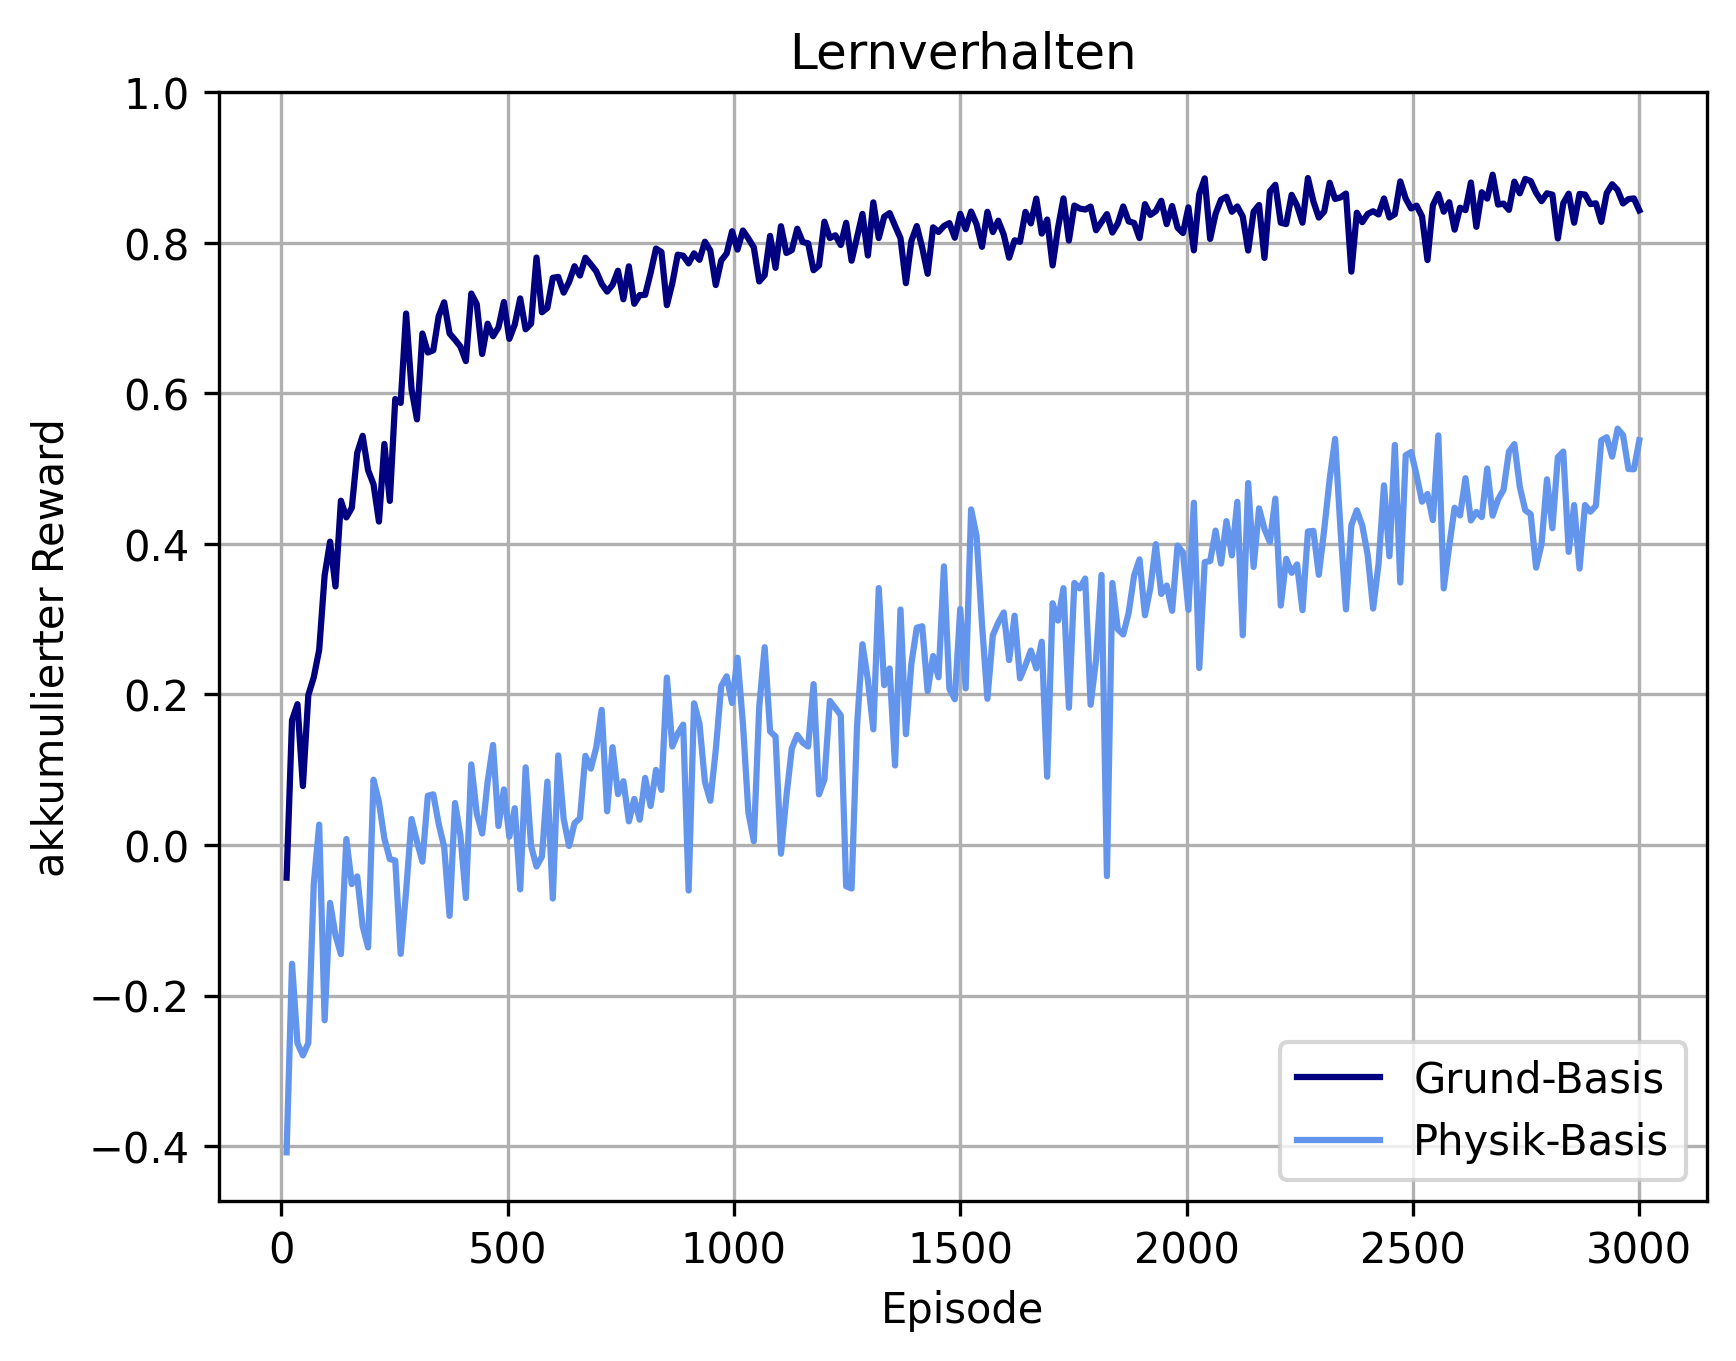
\includegraphics[width=\textwidth-2cm]{images/diskussion/learnplot.png}
    \caption{Akkumulierter Reward zu jeder Episode (Lernverhalten) der Grund-Basis Version und der Physik-Basis Version (eigene Abbildung)}\label{fig:learnplot}
\end{figure}


\subsection{Verwendung von Git und GitHub}\label{sub:d_reflex_git} Die
Verwendung von Git und Github (siehe \doubleref{chap:t_git}) erleichtert die
Arbeit an einem Projekt von dieser Grösse massgeblich. Die Programme ermöglichen
einfache Zusammenarbeit am Programmcode und an der Dokumentation. GitHub dient
dabei zusätzlich als Hilfsmittel zur Organisation durch die integrierte Funktion
der Project Boards. Diese Funktion hätte allerdings zu grösserem Ausmass
Verwendung finden können.

Die Funktion der Branches und Commits von Git wurden durch die Arbeit hindurch
konsequent verwendet. Dabei wurde die Git Flow Arbeitsweise, abgesehen von den
Release Branches und den Hotfix Branches, angewendet (siehe
\doubleref{sub:t_git_git}) Neben den Feature Branches wurden ausserdem
Dokumentation Branches eingeführt. In jedem Dokumentation Branch wurde ein
Kapitel der Dokumentation verfasst. Für die Zusammenführungen der wichtigsten
Branches wurde das Prinzip der Pull Request (siehe \doubleref{sub:t_git_gh})
angewendet. Die Pull Request musste dabei für jeden Branch von demjenigen Autor
akzeptiert werden, der die Pull Request nicht stellte.

Ein weiterer Vorteil von Git und Github ist die Zugänglichkeit des Projektes.
Das gesamte Projekt ist unter folgendem Link einsehbar:
\url{https://github.com/LarsZauberer/Nachzeichner-KI}. Im Projektordner sind
vortrainierte Variationen der künstlichen Intelligenz enthalten. Das Projekt auf
GitHub erfährt möglicherweise Erweiterungen, die in dieser Arbeit nicht mehr
erfasst sind.
